\documentclass[12pt, a4paper]{article}
\usepackage{url}
\usepackage{titlesec}%subsubsubsection
\usepackage{tocloft}%subsubsubsection içindekilerde tanımlamak
\usepackage[utf8]{inputenc}
\usepackage[T1]{fontenc}
\usepackage{graphicx}
\usepackage{amsmath} % For \text and other math environments
\usepackage{amssymb} % For \mathbb
\usepackage{amsfonts} % For \mathbb, if amssymb is not used
\usepackage{bookmark}
\graphicspath{ {./images/} }
\usepackage[ddmmyyyy]{datetime}
\usepackage{pdflscape}
\usepackage{hyperref}%url atıf
\linespread{1.5}
\usepackage[none]{hyphenat}
\sloppy
\usepackage{tikz}
\usepackage{caption} % Tablo başlıkları için
\hypersetup{
	colorlinks=true,
	citecolor=black,
	urlcolor=black,
	linkcolor=black
}


\renewcommand{\dateseparator}{.}
\renewcommand{\contentsname}{İçindekiler}
\renewcommand{\figurename}{Şekil}
\renewcommand{\refname}{Kaynakça}
\renewcommand{\tablename}{Tablo}

\setcounter{secnumdepth}{4} % Derinlik sayacını ayarla, 4 seviyede başlıkları numaralandırmak için
\setcounter{tocdepth}{4} % Derinlik sayacını ayarla, 4 seviyede içindekiler tablosunda göstermek için

\titleformat{\subsubsubsection}
{\normalfont\normalsize\bfseries}{\thesubsubsubsection}{1em}{}
\titlespacing*{\subsubsubsection}
{0pt}{3.25ex plus 1ex minus .2ex}{1.5ex plus .2ex}

\makeatletter
\newcounter{subsubsubsection}[subsubsection]
\renewcommand\thesubsubsubsection{\thesubsubsection.\@arabic\c@subsubsubsection}
\newcommand\subsubsubsection{\@startsection{subsubsubsection}{4}{\parindent}
	{3.25ex \@plus1ex \@minus .2ex}
	{-1em}
	{\normalfont\normalsize\bfseries}}
\newcommand*\l@subsubsubsection{\@dottedtocline{3}{10em}{4em}}
\newcommand*{\subsubsubsectionmark}[1]{}
\makeatother

\title{\textbf{Yapay Zeka Tabanlı Ses Üretimi}\large }
\author{\textbf{Beyzanur Dağdelen}\large}
\date{\textbf{\today}}

\makeatletter         
\def\@maketitle{
	\textbf{\large{KÜTAHYA SAĞLIK BİLİMLERİ ÜNİVERSİTESİ}\centering}\\[4ex]
	\centering
	
\includegraphics[width = 40mm]{ksbu.png}\\[8ex]
	\begin{center}
		{\large \bfseries \@title }\\[4ex] %\Huge
		{\small  \@author}\\[3ex] 
		\section*{\centering Final Raporu}
		\vspace{2\baselineskip}
		
		{\large \bfseries \subitem}
		\section*{\centering Danışman}
		\section*{\small \centering Dr.Öğr.Üyesi Emre Güngör}
		\section*{\small Yapay Zeka \& Veri Odaklı Sistem Tasarımı \& Latex İle Rapor Hazırlama}
		\vspace{2\baselineskip}
		\@date 
\end{center}}
\makeatother


\begin{document}
	
	\maketitle
	
	\thispagestyle{empty}
	
	\newpage
	\tableofcontents  %içindekiler
	\pagenumbering{arabic}
	\newpage
	
	\section*{Özet }
	
	\vspace*{1\baselineskip}
	
	Son yıllarda, derin öğrenme modelleri, doğal dil işleme ve görüntü işleme gibi çeşitli alanlarda önemli ilerlemeler kaydetmiştir. Bu modeller, büyük miktarda veriden öğrenme ve karmaşık görevleri gerçekleştirme yeteneğine sahiptir.

	\vspace*{1\baselineskip}
	
	Ses üretimi, insan-bilgisayar etkileşimi ve sanal gerçeklik gibi birçok uygulamada önemli bir rol oynamaktadır. Geleneksel ses üretim yöntemleri, genellikle sentetik ve gerçekçi olmayan sesler üretmektedir.Özellikle, üretici adversarial ağlar (GAN'ler) ve varyasyonel otoenkoderler (VAE'ler) ses verilerinin işlenmesi ve üretilmesi konusunda güçlü araçlar olarak öne çıkmaktadır.
	
	\vspace*{1\baselineskip}
	
	Bu çalışma, üretici ağlardan VAE kullanarak daha doğal ve gerçekçi sesler üretebilmeyi sunmaktadır.
	
	\vspace*{1\baselineskip}
	
	Bu çalışmanın amacı, birkaç ses dataseti üzerinde eğitilmiş bir VAE modelinin, verilen girişlere göre gerçekçi ve kaliteli ses çıktıları üretebilme yeteneğini incelemektir.
	
	\vspace*{1\baselineskip}
	
	Belirli bir ses datasetini kullanarak VAE modeli eğitilmiş ve modelin çıktıları çeşitli metriklerle değerlendirilmiştir. 	
	
	\vspace*{2\baselineskip}
	\section*{\small \textbf{Anahtar kelimeler}}
	\begin{itemize}
		\small{
			\item Varyasyonel Otoenkoder
			\item Üretici Ağlar
			\item Ses Üretimi
			\item Derin Öğrenme
			\item Ses Dataseti
			\item Yapay Zeka
		}
	\end{itemize}
	\section{Giriş}
	\vspace*{1\baselineskip}
	\raggedright Bu proje, yapay zeka ile ses üretimine odaklanan üç farklı çalışmayı incelemektedir. İlk olarak OpenAI Jukebox projesi, ardından Valerio Velardo'nun "The Sound of AI" YouTube kanalındaki proje ve son olarak Kaggle üzerindeki müzik üretim projesi ele alınacaktır.
	
	Projenin ilk haftasında, yapay zeka ile ses üretimi ve sanal gerçeklik teknolojisi kullanılarak insanları huzurlu hissettiren ortamlar yaratılacaktır. Hedef, iyileştirici etkiye sahip farklı frekanslardaki sesleri yapay zeka ile üreterek, insanların olumsuz duygularını azaltmak ve motivasyon sağlayarak hayatlarını iyileştirmektir.
	
	Bu hedeflere ulaşmak için, VQ-VAE (Vector Quantized-Variational Autoencoder) gibi ileri yapay zeka tekniklerinden faydalanılabilir. VQ-VAE, seslerin temsili ve yeniden oluşturulmasında kullanılabilir. Bu teknik, seslerin duygusal etkilerini analiz ederek, kullanıcıların duygusal durumlarını iyileştirmek için özelleştirilmiş sesler oluşturabilir. Ayrıca, bu seslerin Unreal Engine gibi sanal gerçeklik ortamlarında kullanılmasıyla, kullanıcılar huzur ve motivasyon sağlayan görsel ve işitsel deneyimler yaşayabilirler. Böylece, VQ-VAE ve sanal gerçeklik teknolojileri bir araya getirilerek, insanların duygusal refahlarını artırmak için yenilikçi bir yaklaşım sunulabilir.
	
	\section{Literatür Araştırması}
	Bu bölüm, yapay zeka ile ses üretimine odaklanan üç çalışmayı incelemektedir: OpenAI Jukebox, Valerio Velardo'nun "The Sound of AI" YouTube kanalı ve Kaggle üzerindeki müzik üretim projeleri. Projenin amacı, yapay zeka ve sanal gerçeklik teknolojilerinin birleşimiyle iyileştirici etkileri olan sesler üretmek ve bu sesleri kullanıcıların duygusal refahını artırmak için kullanmaktır. VQ-VAE (Vector Quantized-Variational Autoencoder) tekniği, bu seslerin temsili ve yeniden oluşturulmasında kullanılacak ve özelleştirilmiş sesler oluşturulacaktır. Bu sesler, Unreal Engine gibi sanal gerçeklik ortamlarında kullanılarak kullanıcılar için huzur ve motivasyon sağlayan deneyimler sunacaktır.
	
	\subsection*{OpenAI Jukebox}
	OpenAI Jukebox, insan yapımı şarkılara benzeyen yeni müzik parçaları üretebilen bir yapay zeka projesidir. Derin öğrenme algoritmaları kullanarak geniş bir müzik veri kümesi üzerinde eğitilmiş olan model, çeşitli müzik türlerinde ve tarzlarda orijinal parçalar oluşturabilir. Jukebox, sadece melodiler ve armoniler değil, aynı zamanda şarkı sözleri de üretebilir. Kullanıcılar, belirli bir sanatçı, tür veya ruh hali gibi kriterlere göre müzik oluşturmak için Jukebox'ı yönlendirebilirler. Jukebox'ın dikkat çeken özellikleri arasında geniş müzik yelpazesi, şarkı sözleri üretme yeteneği, kullanıcı tarafından özelleştirilebilir olması ve yüksek kaliteli sonuçlar yer almaktadır. Bu proje, müziğin sınırlarını genişletirken yapay zeka alanında büyük bir ilerleme sunmaktadır\cite{jukebox}.
	
	\subsection*{Valerio Velardo'nun "The Sound of AI" YouTube Kanalı}
	Valerio Velardo'nun "The Sound of AI" isimli YouTube kanalındaki proje, sinir ağlarıyla ses oluşturma konusunu ele almaktadır. Bu projede, değişken otomatik kodlayıcılar kullanarak ses üretimi ve eğitim süreçleri tanıtılmaktadır. TensorFlow ve Keras kullanarak kodlama yapmanın yanı sıra, ses veri setlerinin ön işlenmesi ve kısa süreli Fourier dönüşümü gibi işlemler de detaylı olarak anlatılmaktadır. Velardo'nun projesi, varyasyonel oto-kodlayıcılarla ses üretimi, gerekli ön bilgiler ve kullanılacak teknoloji yığını hakkında kapsamlı bilgiler sunar. Proje, Python, TensorFlow, Keras ve Librosa gibi araçlar kullanılarak uygulamalı ve teorik bilgilerle desteklenmektedir\cite{vvAi}.
	
	\subsection*{Kaggle Üzerindeki Müzik Üretim Projesi}
	Kaggle üzerindeki proje, OpenAI Jukebox araştırma makalesinden ilham alınarak geliştirilmiştir \cite{kaggleCode}. Bu projede, belirli müzik kategorilerinden (jazz ve klasik müzik) müzik üretebilecek bir varyasyonel oto-kodlayıcı modeli geliştirilmiştir. Model, TensorFlow kullanılarak uygulanmış ve ses işlemleri için Librosa kütüphanesi kullanılmıştır. Proje, varyasyonel oto-kodlayıcıların çalışma prensiplerine, kısa süreli Fourier dönüşümüne ve ses veri setlerinin ön işlenmesine odaklanmaktadır. Model, müzik üretimi için optimize edilmiş olup, gelecekte daha fazla müzik kategorisi ile eğitilerek daha geniş bir yelpazede müzik üretebilecek şekilde geliştirilebilir. Bu projede, yapay zekanın müzik üretiminde nasıl kullanılabileceği ve varyasyonel oto-kodlayıcıların potansiyeli üzerinde durulmuştur.
	
	Bu üç çalışma, yapay zeka ile ses üretiminin farklı yönlerini ve uygulamalarını ele alarak, projenin temelini oluşturmaktadır. Yapay zeka ve sanal gerçeklik teknolojilerinin entegrasyonu ile iyileştirici etkileri olan sesler üretmek ve bu sesleri kullanıcıların duygusal refahını artırmak için kullanmak mümkündür. Bu çalışmalar, seslerin duygusal etkilerini analiz etmek ve özelleştirilmiş sesler oluşturmak için gerekli teknik ve teorik bilgileri sağlamaktadır.


	\subsection{Ses Datasetleri} 	
	\begin{itemize}
		\item N-synth
		\item MAESTRO
	\end{itemize}
	
	\subsubsection{N-synth} 
	Benzersiz perde ve tınıya sahip 305.979 müzik notası içeren, tek seferlik enstrümantal notalardan oluşan bir veri kümesidir. Sesler, ticari örnek kütüphanelerindeki 1006 enstrümandan toplanmıştır ve kaynaklarına (akustik, elektronik veya sentetik), enstrüman ailesine ve sonik niteliklerine göre açıklanmıştır. Açıklamada kullanılan enstrüman aileleri bas, pirinç, flüt, gitar, klavye, tokmak, org, kamış, yaylı, synth lead ve vokaldir. Enstrümanlar için dört saniyelik monofonik 16kHz ses parçacıkları (notalar) oluşturulmuştur \cite{nsynth}.
	
	\subsubsection{MAESTRO} 	
	MAESTRO (MIDI and Audio Edited for Synchronous Tracks and Organization), nota etiketleri ve ses dalga formları arasında ince bir hizalama (~3 ms) ile yakalanan 200 saatin üzerinde virtüöz piyano performansından oluşan bir veri kümesidir \cite{maestro}.  
	MIDI, dijital enstrümanların birbirleriyle 'mesajlar' aracılığıyla iletişim kurmasını sağlayan bir protokoldür. Bu mesajlar, çalma için kullanılacak enstrümanın türü, çalınacak notalar, bir notanın ne zaman başlayacağı, bir notanın ne zaman biteceği vb. hakkında bilgi depolar.
	\vspace*{2\baselineskip}
	
	
	\subsection{Kaglle Kodu İle Kullanılan Datasetler} 	
	\vspace*{1\baselineskip}
	\begin{itemize}
		\item FSDD-Free Spoken Digit Dataset
		\item Gunshot Audio Dataset
	\end{itemize}
	\subsubsection{FSDD - Free Spoken Digit Dataset}
	Free Spoken Digit Dataset (FSDD), 8kHz'de wav dosyalarında konuşulan rakamların kayıtlarından oluşan basit bir ses/konuşma veri kümesidir. Kayıtlar, başlangıçlarında ve sonlarında neredeyse minimum sessizliğe sahip olacak şekilde kırpılmıştır. Bu veri seti 6 konuşmacıdan, 3.000 kayıttan (konuşmacı başına her rakamdan 50 adet) ve İngilizce telaffuzlardan veri içermektedir \cite{fsdd}.
	\vspace*{1\baselineskip}
	
	
	8kHz'de wav dosyalarında konuşulan rakamların kayıtlarından oluşan basit bir ses/konuşma veri kümesidir. Kayıtlar, başlangıç ve bitişlerinde neredeyse minimum sessizliğe sahip olacak şekilde kırpılmıştır.
	
	FSDD açık bir veri setidir.
	
	Mevcut durum
	\begin{itemize}
		\item 6 hoparlör
		\item 3.000 kayıt (konuşmacı başına her rakamdan 50 adet)
		\item  İngilizce telaffuzlar
	\end{itemize}
	
	
	Organizasyon:
	Dosyalar aşağıdaki formatta adlandırılır: \newline
	{digitLabel}\_{speakerName}\_{index}.wav \newline Örnek: 7\_jackson\_32.wav
	
	
	\vspace*{2\baselineskip}
	\subsubsection{Gunshot Audio Dataset}
	
	Veri kaynağı olarak YouTube kullanılmaktadır. Silah seslerini toplamak için değişken ortam modeli kullanılmıştır. Silah modellerinin sesleri YouTube üzerinden herkese açık olan videolar kullanılarak toplanmıştır. Farklı tarihlerde toplanan bu dosyalar indirilerek her silah tipi için 2 saniyelik parçalar üretilmiştir. Bu şekilde 8 silah modeli ile toplam 851 dosya tipi elde edilmiştir. Ses dosyalarının örnekleme hızı 44100 Hz'dir. Öncelikle her bir ses dosyası wav dosya formatına dönüştürülmüştür. Daha sonra sesler dikkatlice dinlenmiş ve içerisinde farklı sesler veya gürültüler olmadığından emin olunmuştur. Ses dosyalarının parçalanması sırasında aynı sesin tekrar tekrar devam etmediği dikkatlice kontrol edilmiştir. Tüm bu işlemler için WavePad Audio Editor programı kullanılmıştır. Tablo 1'de oluşturulan seslerin sayısına ilişkin detaylar listelenmiştir \cite{gunshot}.
	
	Toplanan silah ses veri setinin detayları
	
	\begin{table}[ht!]
		\caption{Silah Ses Verisi}
		\raggedright
		\label{tablo:silah_ses_verisi}
		\centering
		\begin{tabular}{|c|c|c|}
			\hline
			\textbf{Kimlik} & \textbf{Model} & \textbf{Gözlem Sayısı} \\
			\hline
			1 & AK-47 & 72 \\
			\hline
			2 & IMI Desert Eagle (Çöl Kartalı) & 100 \\
			\hline
			3 & AK-12 & 98 \\
			\hline
			4 & M16 & 200 \\
			\hline
			5 & M249 & 99 \\
			\hline
			6 & MG-42 & 100 \\
			\hline
			7 & MP5 & 100 \\
			\hline
			8 & Zastava M92 & 82 \\
			\hline
		\end{tabular}
	\end{table}


	\section{Yöntem}
		Bu projede, derin öğrenme alanında öne çıkan ve çeşitli uygulamalarda başarıyla kullanılan VAE (Variational Autoencoder) ve türevleri araştırılmıştır. Araştırmalar sonucu VAE kullanılmıştır. Üretici ağlar olarak bilinen bu modeller, veri üretimi ve temsili öğrenme konularında güçlü araçlar sunmaktadır. Projede ayrıca, model performansını artırmak ve en iyi sonuçları elde etmek amacıyla çeşitli optimizasyon algoritmaları ( Adam ) kullanılmıştır. Kullanılan loss fonksiyonları (KL Diverjansı) ise, modelin doğruluğunu ve genelleme yeteneğini maksimize etmek için özenle seçilmiş ve optimize edilmiştir. Bu yöntemler, projenin hedeflerine ulaşmasında ve başarılı sonuçlar elde edilmesinde kritik rol oynamıştır.
			\vspace*{1\baselineskip}
			\subsection{Variational Autoencoder (VAE): Yaratıcı ve Esnek Veri Üretimi}
			Variational Autoencoder (VAE), veri temsilini öğrenmek ve yaratıcı bir şekilde yeni veri noktaları üretmek için kullanılan önemli bir modeldir.
			
			VAE, derin öğrenme modelleri sınıfında yer alan bir tür yapay sinir ağıdır. Amacı, veri setindeki örüntüleri öğrenerek, veriyi daha az boyutta bir temsile sıkıştırmak ve bu temsili kullanarak yeni veri noktaları oluşturmaktır. Genellikle denetimsiz öğrenme yöntemi olarak kullanılan VAE, veri setinin içsel yapısını anlama yeteneğine sahiptir \cite{VAE}.
			
			\subsubsubsection{VAE’nin İşlevi ve Autoencoder (AE) ile Farkı}
			VAE, geleneksel bir autoencoder (AE) gibi çalışır, ancak belirgin bir farklılık bulunur. AE, gizli bir temsil (latent representation) oluşturmak için veriyi sıkıştırır ve ardından bu temsil aracılığıyla veriyi yeniden oluşturur. VAE ise sadece veriyi sıkıştırmakla kalmaz, aynı zamanda verinin olası dağılımını modelleyerek, veri noktalarının olasılık dağılımını öğrenir. Bu da VAE’nin veri üretiminde daha esnek ve çeşitlilik yaratabilme yeteneğine sahip olmasını sağlar.
			
			\subsubsection{VAE’nin Çalışma Prensibi}
			VAE’nin temel prensibi, veriye gizli bir yapısal temsil oluşturmak ve bu temsil aracılığıyla yeni veri noktaları üretmektir. Bu süreç iki ana bileşen üzerine kuruludur: encoder ve decoder.
			\vspace*{1\baselineskip}
			Veriyi latent uzayın parametreleri olan bir dağılımın parametreleri haline getiren encoder ağıdır. Bu dağılım genellikle Gaussian (normal) dağılımı olarak belirtilir. Encoder, veriyi sıkıştırarak, her bir veri noktasını latent uzayın içindeki bir noktaya eşler.
			\vspace*{1\baselineskip}	
			Latent uzaydaki noktaları orijinal veriye çeviren ise decoder ağıdır. Encoder tarafından elde edilen latent uzay temsilini alır ve bu temsili orijinal veriye dönüştürür.
			
			\subsubsection{GAN ile Bağlantısı}
			GAN, gerçekçi veri üretmek için kullanılırken, VAE daha yapılandırılmış ve kontrollü bir şekilde veri üretir. Bazı çalışmalar, VAE’nin öğrendiği temsili GAN yapısında kullanarak daha kaliteli ve çeşitli veri üretimi sağladığını göstermiştir.
			
			\subsubsection{Kullanım Alanları}
			Kullanım alanları geniş olan VAE’ye şunlar örnek verilebilir:
			\begin{itemize}
				\item Görüntü ve Video İşleme: Görüntü tamamlama, yeniden oluşturma ve sentezleme işlemlerinde kullanılabilir.
				\item Doğal Dil İşleme: Dil modelleme, metin üretimi ve dilin öğrenilmesi gibi alanlarda kullanılabilir.
				\item 	Yaratıcı İçerik Üretimi: Sanat, müzik ve edebiyat gibi yaratıcı içeriklerin oluşturulmasında kullanılabilir.
			\end{itemize}
			
			Variational Autoencoder, derin öğrenme ve generatif modelleme alanındaki önemli bir gelişmedir. Verinin daha esnek bir temsilini öğrenerek hem veri üretiminde kullanılabilirliği hem de verinin içsel yapısını anlama yeteneği ile birçok alanda geniş bir kullanım potansiyeline sahiptir.
			
			\clearpage
			\subsubsection{VAE \& VQ-VAE \& VAE-GAN}
			Yapay zeka tabanlı model türleri olan bu üç model, özellikle ses ve görüntü üretmede kullanılırlar \cite{vaeTypes}.
			\begin{figure}[!htb]
				\centering
				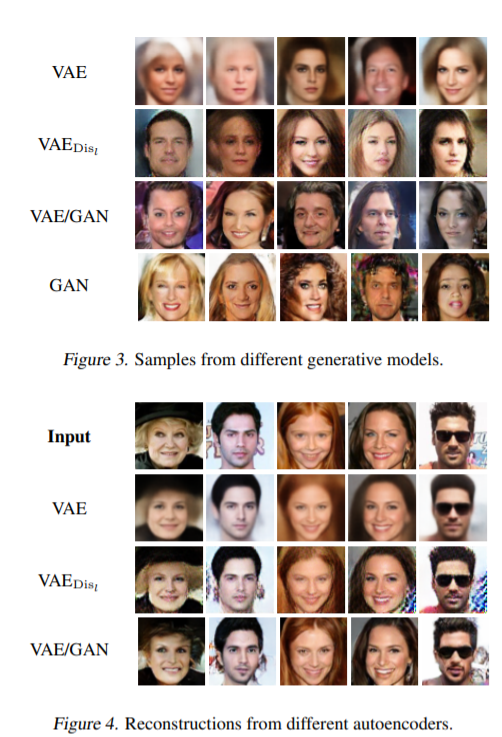
\includegraphics[width=.8\linewidth]{models.png}
				\caption{query\&output}\label{Fig:Data1}\cite{vaeTypes}
			\end{figure}
			\subsubsubsection{VAE}
			Vanilya VAE en iyi bilinen üretken modellerden biridir (GAN dışında). Bir aşağı örnek, genellikle z olarak adlandırılan bir gizli vektör ve bir yukarı örnekten oluşan üç bölümü vardır. Aşağı örnek\ref{Fig:Data2} genellikle konvolüsyonlardan oluşur ve yukarı örnek ya transpoze edilmiş bir konvolüsyondur ya da normal bir yukarı örnek ve yukarı örnekten tutulan uzamsal boyutlarla konvolüsyon içeren bir bloktur. Bununla birlikte, konvolüsyonlu yukarı örnekleme genellikle normal transpoze konvolüsyonlardan daha düzgün sonuçlar üretir.
			\begin{figure}[!htb]
				\centering
				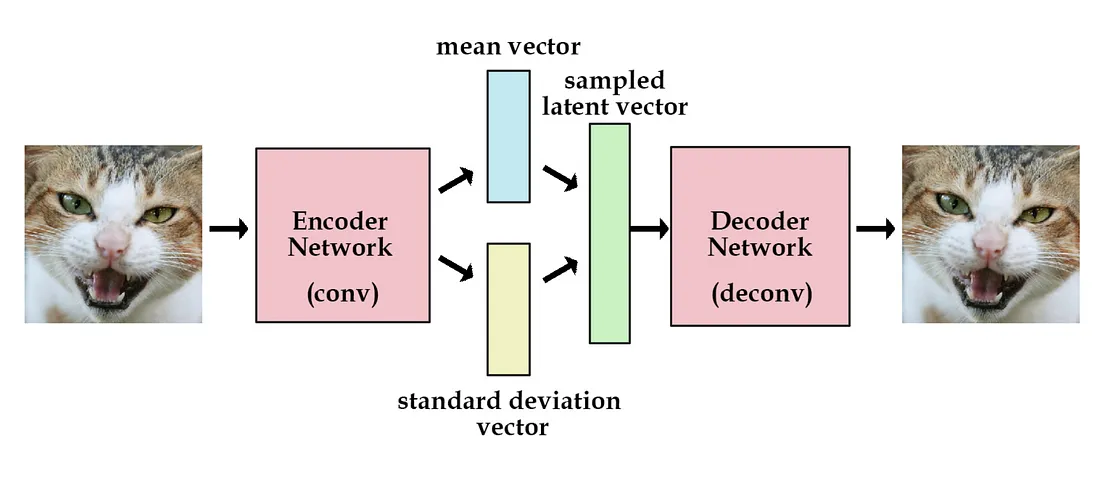
\includegraphics[width=.7\linewidth]{vae.png}
				\caption{VAE}\label{Fig:Data2} \cite{vaeTypes}
			\end{figure}
			
			\subsubsubsection{VQ-VAE}
			VQ-VAE, vanilya VAE'nin ayırt edici özelliği olan gizli uzayın yeniden yaratılmasıdır. Bu, gizli uzayı ortadan kaldırmak anlamına gelmemektedir, sadece sürekli yerine ayrık olmasına izin verir, dolayısıyla adın Vektör Niceleme VAE'dir. Gizli uzaydaki noktalar VQ-VAE'de ayrıktır ancak VAE'de süreklidir \cite{vqvae}.
			
			\begin{figure}[!htb]
				\centering
				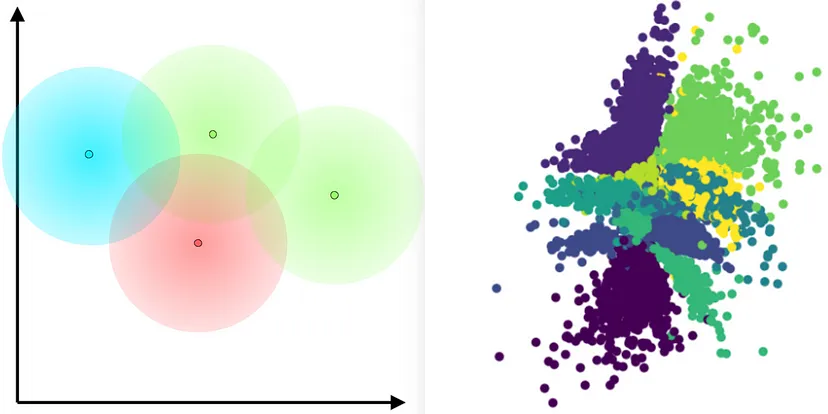
\includegraphics[width=.3\linewidth]{vqvae.png}
				\caption{VQ-VAE}\label{Fig:Data3}\cite{vqvae}
			\end{figure}
			
			En yakın embeddingi ya da gizli uzayda örnekleme yapılacak en yakın noktayı hesaplayan bir fonksiyon ekleyerek bulanık çıktılar sorununu çözülmesi hedeflenmektedir. Çünkü VQ-VAE eğitildiği bir noktadan örnekleme alınırsa daha keskin olacaktır.
			VQ-VAE 2 görüntü kalitesi ve çoklu nesil çeşitliliği ölçütlerinde BIG-GAN'ı geride bırakmıştır. Bununla birlikte, aynı sonucu elde etmenin bir başka yolu da GAN'ın discriminatorunu kullanmaktır.
			
			\subsubsubsection{VAE-GAN}
			GAN'lar bazen insanları bile kandırabilecek hiper-gerçekçi görüntüler üretebilmektedir fakat amaçlanan özelliklere sahip görüntüler üretmek için VAE'nin gizli uzay gibi bazı kısımlarına hala ihtiyaç duyulabilmektedir. Bunu yapmak için, GAN'ın ayırt edicisini VAE'nin dönüştürülmüş konvolüsyonlarından sonra eklemelidir. Görüntülerin daha keskin ve daha gerçekçi olmasına yardımcı olmak için VAE'nin loss fonksiyonuna bir ayırıcı kayıp bileşeni eklenmelidir \cite{vaegan}.
			\begin{figure}[!hb]
				\centering
				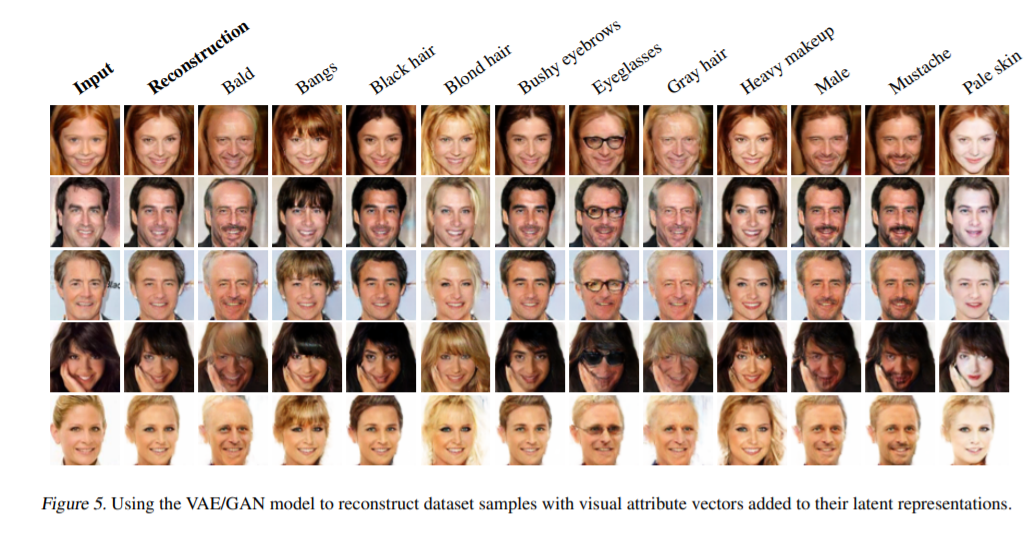
\includegraphics[width=.5\linewidth]{vaegan.png}
				\caption{VAE-GAN}\label{Fig:Data4}\cite{vaeTypes}
			\end{figure}
			\clearpage
			
			%2.HAFTA___ Entropi \& KL Divergence \& Unreal Enginede Makro
			
			\subsection{Entropi} 	
			Entropi(düzensizlik), bir olayın veya iletinin içerdiği bilgi miktarıdır \cite{entropi}. Bilgiyi ise bilgisayarlarda bitler halinde depolanır. Bilginin depolama işlemi gerçekleştirilirken minimum bit sayısı olacak şekilde saklanması amaçlanır. Olayların gerçekleşme olasılığı ile içerdiği bilgi miktarı karşılaştırılırsa;
			
			\begin{itemize}
				\item Düşük olasılıklı gerçekleşen olaylar büyük miktarda bilgi içermektedir.
				\item  Yüksek olasılıkla gerçekleşen olaylar az sayıda bilgi içermektedir.
			\end{itemize}
			
			Bir olayın içerdiği bilgi miktarını formülize adildiğinde aşağıdaki(\ref{bilgi_miktari}) formül elde edilir.
			
			\begin {center}
				\begin{equation}
					Bilgi(x) = -log_2(p(x))
					\label{eqn: bilgi_miktari}\cite{entropi}
				\end{equation}
			\end {center}
			
			\vspace*{1\baselineskip}
			Hilesiz bir madeni para için para yazı-tura oyunu için havaya atıldğında aşağıdaki tablo ortaya çıkmaktadır(\ref{tab:Tablo1}).
		
		
			\begin{table}[htbp]
				\begin {center}
				\caption{Hilesiz Para Örneği \cite{entropi}}	\label{tab:Tablo1}
				
				\begin{tabular}{|l|l|l|}
					\hline
					Çıktılar & Yazı & Tura \\
					\hline
					Olasılık & 0.5 & 0.5 \\
					\hline
					Bit Gösterimi & 0 & 1 \\
					\hline
					Bit Sayısı & \multicolumn{2}{|c|}{1} \\
					\hline
					Bilgi: $H(p)= -log_2(p(x))$	& 1 & 1 \\
					\hline 
				\end{tabular}
				\vspace*{1\baselineskip}
				\end {center}
			\end{table}
		
			Bu olayların gerçekleşme olasılığı eşit olduğundan olaya dahi taşıdıkları bilgi miktarları birbirine eşit ve 2'dir.
			
			Madeni para hileli olduğunda yazı ve tura gelme olasılıkları eşit değildir(\ref{tab:Tablo2}). 
			\begin{table}[htbp]
				\begin {center}
				\caption{Hileli Para Örneği \cite{entropi}}	\label{tab:Tablo2}
				\begin{tabular}{|l|l|l|}
					\hline
					Çıktılar & Yazı & Tura \\
					\hline
					Olasılık & 0.25 & 0.75 \\
					\hline
					Bit Gösterimi & 0 & 1 \\
					\hline
					Bit Sayısı & \multicolumn{2}{|c|}{1} \\
					\hline
					Bilgi: $H(p)= -log_2(p(x))$	& 2 & 0.415 \\
					\hline
				\end{tabular}
				\end {center}
			\end{table}
		
			Hilesiz 2 adet bağımsız madeni paranın değerleri aşağıdaki gibidir(\ref{tab:Tablo3});
			\begin{table}[htbp]
				\begin {center}
				\caption{Hileli Para Örneği \cite{entropi}}	\label{tab:Tablo3}
				\begin{tabular}{|l|l|l|l|l|}
					\hline
					Çıktılar & Yazı-Yazı & Yazı-Tura & Tura-Yazı & Tura-Tura \\
					\hline
					Olasılık & 0.25 & 0.25 & 0.25 & 0.25\\
					\hline
					Bit Gösterimi & 00 & 01 & 10 & 11 \\
					\hline
					Bit Sayısı & \multicolumn{4}{|c|}{2} \\
					\hline
					Bilgi: $H(p)= -log_2(p(x))$	& 2	& 2 & 2	& 2 \\
					\hline
				\end{tabular}
				\end {center}
			\end {table}
		
			Olasılıkları farklı olan 4 olayı incelendiğinde(\ref{tab:Tablo4});
			\begin{table}[!ht]
				\begin {center}
				\caption{Hileli Para Örneği \cite{entropi}}	\label{tab:Tablo4}
				\begin{tabular}{|l|l|l|l|l|}
					\hline
					Çıktılar & $X_1$ & $X_2$ & $X_3$ & $X_4$ \\
					\hline
					Olasılık & 0.5 & 0.25 & 0.125 & 0.125\\
					\hline
					Bit Gösterimi & 1 & 01 & 000 & 001 \\
					\hline
					Bit Sayısı & 1 & 2 & 3 & 3  \\
					\hline
					Bilgi: $H(p)= -log_2(p(x))$	& 1 & 2 & 3 & 3 \\
					\hline
				\end{tabular}
				\end {center}
			\end{table}
			\newline
				\vspace*{5\baselineskip}
			Burada bit gösterimlerinin ve sayılarının farklı olduğu gözükmektedir. Burada olaylar 3’e ayrılmış gibi görülebilmektedir. Yani p: olayın gerçekleşme olasılığı gösterilirse(\ref{eqn: p_olayının_gerçekleşme_olasılığı});
			
			\begin{equation}[!hb]
				P(X_1) = P(x_2) + P(x_3) + P(x_4)
			\end{equation}
			
			\begin{equation}[!ht]
				P(x_2) = P(x_3) + P(x_4)
				\label{eqn: p_olayının_gerçekleşme_olasılığı}
			\end{equation}
		
			şeklindedir. 
				
			İçerdikleri bilgi miktarlarına bakıldığında gerçekleşme olasılığı düşük olan olayların daha yüksek bilgi içerdikleri gözükmektedir.
			
			İçerdiği bilgi hesaplamasını rastgele bir X değişkeni için hesaplarsak tüm gerçekleşen olaylar üzerinden beklenen bilgiye(expected information) bakılmaktadır. Entropi formüllerinden birisi olan Shannon Entropi aşağıdaki şekildedir(\ref{Shannon Entropisi}).
			\begin {center}
			\begin{equation}H(X) = - \sum_{i=1}^{n}p_i log_2 p_i	\label{eqn:Shannon Entropisi}
			\end{equation}
			\end {center}
			Sırayla bir adil ve bir adil olmayan madeni paraların yazı tura olaylarının entropileri ise(\ref{tablo5});\newline
				\begin{table}[!ht]\begin{minipage}{0.4\textwidth}
				\begin {center}
				\caption{ Bir Adil Madeni Para Örneği \cite{entropi}}	\label{tab:tablo5}
				\begin{tabular}{|l|l|l|}
					\hline
					Çıktılar & Yazı & Tura \\
					\hline
					Olasılık & 0.5 & 0.5 \\
					\hline
					Bit Gösterimi & 0 & 1 \\
					\hline
					Bit Sayısı & \multicolumn{2}{|c|}{1} \\
					\hline
					Bilgi: $H(p)= -log_2(p(x))$	& 1 & 1 \\
					\hline
					Entropi: $:p* -log_2(p(x))$	& 0.5 & 0.5  \\
					\hline
					Beklenen Entropi& \multicolumn{2}{|c|}{1}  \\
					\hline
				\end{tabular}
				\end {center}
			\end{minipage}\hfill
			\begin{minipage}{0.4\textwidth}
			
					\begin {center}
					\caption{Bir Adil Olmayan Para Örneği \cite{entropi}}	\label{tab:Tablo6}
				\begin{tabular}{|l|l|l|}
					\hline
					Çıktılar & Yazı & Tura \\
					\hline
					Olasılık & 0.25 & 0.75 \\
					\hline
					Bit Gösterimi & 0 & 1 \\
					\hline
					Bit Sayısı & \multicolumn{2}{|c|}{1} \\
					\hline
					Bilgi: $H(p)= -log_2(p(x))$	& 2 & 0.415 \\
					\hline
					Entropi: $:p*	 -log_2(p(x))$	& 0.5 & 0.307  \\
					\hline
					Beklenen Entropi& \multicolumn{2}{|c|}{0.807}  \\
					\hline
				\end{tabular}\label{tablo6}
				\end {center}
			\end{minipage}\newline
			\end{table}
			Olaydaki belirsizlik, eşit olasılıklı yazı turaya göre daha düşüktür. Yani entropisi daha düşüktür.
			
			P(X) dağılımı Bernoulli dağılımı olarak 2 ayrı x ve y olaylarının gerçekleştiği tanımlanılırsa Bernoulli dağılımı altında $p(x) = 1 — p(y)$ denilebilir. x olayının gerçekleşme olasılığı p(x) e göre entropi fonksiyonunun grafiği ise aşağıdaki şekildedir(\ref{Fig1:grafik});
			\begin {center}
			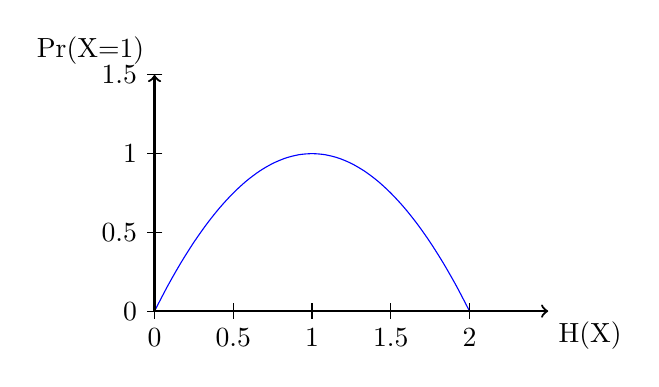
\begin{tikzpicture}
				
				\begin{scope}[scale=2] % Grafiği iki kat büyüt
			
					% Parabol çizimi
					\draw[domain=0:2,smooth,variable=\x,blue] plot ({\x},{-(\x-1)^2 + 1});
					
					% Eksenler
					\draw[thick,->] (0,0) -- (2.5,0) node[anchor=north west] {H(X)};
					\draw[thick,->] (0,0) -- (0,1.5) node[anchor=south east] {Pr(X=1)};
					
					% x eksenindeki çizgiler ve etiketler
					\foreach \x in {0,0.5,1,1.5,2}
					\draw (\x,0.05) -- (\x,-0.05) node[anchor=north] {$\x$};
					% y eksenindeki çizgiler ve etiketler
					\foreach \y in {0,0.5,1,1.5}
					\draw (0.05,\y) -- (-0.05,\y) node[anchor=east] {$\y$};\label{Fig1:grafik}
				\end{scope}
			\end{tikzpicture}
			\end {center}
			
			İki olayın gerçekleşme olasılığı eşit olduğunda (yani p(x)=0=1-p(y) dolayısıyla p(y)=0.5) entropinin maksimum değerini aldığı gözükmektedir. İki olayın gerçekleşme olasılıkları birbirine eşit olduğundan hangi sonucun geleceği diğer durumlara göre daha belirsizdir ve bu yüzden entropi maksimum değeri alır.
			
			\subsection{Çapraz Düzensizlik (Cross-Entropy) ve KL Iraksaklığı (KL Divergence)}
			Cross-Entropy, gerçek olasılık dağılımı P iken bulunan Q olasılık dağılımı için beklenen entropi değeridir. Cross-Entropy formülü	(\ref{CrossEntropy2});
			\begin {center}
			\begin{equation}H(p,q) = - \sum_{x} p(x) log_q(x)	\label{eqn:Cross-Entropy}
			\end{equation}
			\end {center}
			Cross-Entropy’i Kullback-Leibler(KL) ıraksaklığını kullanarak da aşağıdaki şekilde gösterilebilmektedir;
			\begin {center}
		
				\begin{equation}H(p,q) = H(p) + D_w(p | | q)	\label{eqn:CrossEntropy2}	\end{equation}
			\end {center}
			
			H(p), doğru olasılık dağılımı P’nin entropisidir. P doğru olasılık dağılımını bulmak için bir model kurulduğunda P’ye yaklaşık olan Q olasılık dağılımını vermektedir. Bu 2 olasılık dağılımı arasındaki farklılığa bakmak için tanımlanan ölçülerden  biri Cross-Entropy fonksiyonunda gördüğünüz $D_kl(p||q)$ ölçüsü Kullback-Leibler(KL) ıraksaklığıdır.
			
			\subsection{Kullback-Leibler Iraksaklığı \newline (KL-Divergence)}
			Makine öğrenmesi alanında P olasılık dağılımı yerine Q olasılık dağılımı kullanılırken elde edilen bilgi kazanım anlamınındayken, Bayes çıkarımında ise önceki dağılım Q’dan sonraki dağılım P’ye geçerken ki elde edilen bilgi kazanımıdır.Yani P olasılık dağılımını tahmin ederken Q olasılık dağılımı kullanıldığında kaybedilen  bilgi miktarıdır. Formülünün olabilirlik oranından elde edilmesi ise adım adım aşağıdaki şekildedir(\ref{Olabilirlik oranı}).
			\newline
			\begin {center}
				\begin{equation}LR=\frac{p(x)}{q(x)}	\label{eqn:Olabilirlik oranı}	\end{equation}
		
			\end {center}
		
			
			x değeri bilinmeyen bir olasılık dağılımından ise yukarıda görülen (\ref{Olabilirlik oranı}) olabilirlik oranı x örneklemi için P dağılımından gelmenin Q dağılımından gelmeye nazaran ne kadar olası olduğunu göstermektedir. Birden fazla bağımsız örneklemler için olabilirlik fonksiyonu hesaplanılırken her örneklem için bulunan olabilirlik oranının çarpılması gerekmektedir. 
			\begin {center}
			\begin{equation}LR=\prod_{i=0}^{n}\frac{p(x_i)}{q(x_i)}		\end{equation}
				\end {center}
				\begin {center}
			\begin{equation}LR = \sum_{i=0}^{n} log(\frac{p(x_i)}{q(x_i))}	\end{equation}
			\end {center}
			Örneklemde Q dağılımı üzerinde P’ye dair ortalama ne kadar bilgi verdiğini hesaplamak için olabilirlik oranının beklenen değeri\ref{Olasılık dağılımları ayrıkken Kullback-Leibler Iraksaklığı};
				\begin {center}
			\begin{equation}D_kl(P||Q) =  \sum_{i=0}^{n} p(x_i)log(\frac{p(x_i)}{q(x_i))}	\label{eqn:Olasılık dağılımları ayrıkken Kullback-Leibler Iraksaklığı}	\end{equation}
			\end {center}
			
			KL ıraksaklığı formülünü yukarıdaki şekliyle elde etmiş olunmaktadır. KL ıraksaklığının 0 olması P ve Q dağılımlarının aynı olduğunu ifade etmektedir. Yukarıdaki formül P ve Q dağılımları ayrık olasılık dağılımları için kullanılabilir(Örneğin Bernouilli, Poisson, Binom dağılımları).
		
				\begin {center}
			\begin{equation}D_kl(P||Q) =    \int_{-\infty}^{\infty}p(x_i)log(\frac{p(x_i)}{q(x_i))}\,dx \label{eqn: Olasılık dağılımları ayrıkken Kullback-Leibler Iraksaklığı}		\end{equation}
			\end {center}
			Olasılık dağılımları sürekliyse formül yukarıdaki gibi integral şeklinde tanımlanır.
			
			
			%3.HAFTA___Optimizer
			\subsection{Optimizer} 	
			Optimizasyon algoritmaları, modelin kayıp fonksiyonunu minimize ederek modelin daha iyi performans göstermesini sağlar. Bu algoritmalar, ağırlıkları güncellemek için gradyan iniş (gradient descent) ve türev tabanlı teknikler kullanır.
			Optimizatörler, sinir ağı eğitiminde önemli bir rol oynar. Ağırlık ve önyargılar gibi parametreleri ayarlayarak ağın bir fonksiyonu en iyi şekilde temsil etmesini sağlarlar \cite{deep_learning}. 
			\begin{enumerate}
				\item 	Gradyan İniş (Gradient Descent):
				Gradyan İniş (Gradient Descent), belki de en temel optimizasyon algoritmasıdır ve derin öğrenme modellerinin eğitiminde sıkça kullanılır. Amacı, kayıp fonksiyonunun ağırlıklar üzerinden türevini alarak, negatif gradyana doğru ağırlıkları güncellemektir \cite{sgd}.
				
				
				\item	Stochastic Gradient Descent:
				Stokastik gradyan azalma, gradyan azalma gibidir ancak gradyan azalmada bütün veri seti kullanılırken, stokastik gradyan azalmada tek bir örneklem kullanılır. Stokastik gradyan azalma yönteminde tek seçilen veri ile işlem yapıldığı için global mimimum noktasına kararlı bir şekilde ilerleme gözlenmez. Diğer taraftan, rastgele parametre katsayıları ile bir örnek üzerinde işlem yaptığından local minimaya düşme ihtimali daha düşüktür \cite{sgd}.
				
				Stokastik gradyan azalma, gradyan azalmaya nazaran daha gürültülü bir grafik çizer. Minima noktasına ulaşması için daha fazla iterasyon sayısına ihtiyaç duymaktadır ancak tek bir örnek üzerinde çalıştığı için, hesaplama maliyeti gradyan azalmadan daha verimlidir.
				
				
				\item 	Uyarlanabilir Gradyan Algoritması (Adagrad):
				Adagrad, parametre güncellemelerini her bir parametre için ayrı ayrı ölçeklendirerek gradyan iniş optimizatörünün bir modifikasyonudur .
				Minibatch Gradyan azalmada başarıyı etkileyen faktörlerden biride kullanılan adımın boyutuydu. Bu adım boyutunu doğru belirleyememek, bizi minimuma yakınsamama problemi ile karşı karşıya bırakabilirdi. AdaGrad burada devreye girmekte ve adım boyutunu otomatik olarak belirlemektedir \cite{sgd}.
				
				Uyarlanabilir Gradyan Algoritması, gradyan tabanlı optimizasyon için bir algoritmadır. Öğrenme oranı, geçmiş gözlemleri hesaba dahil edilerek parametrelere bileşen olarak uyarlanır. Her parametrenin performansı artıran kendi öğrenme oranı vardır. NLP ve Görüntü tanıma konularında kullanımı uygundur.
				
				
				\item 	Momentum:
				Momentum, Stokastik gradyan azalma ile kullanılan popüler bir tekniktir. Sadece mevcut durumda hesaplanan gradyan değerini kullanmak yerine eski gradyanların değerlerini de kullanarak gideceği yönü belirlemeye çalışır.Salınım yaparak minimuma ulaşmaya çalışmaktadır. Çünkü bir batch için hatayı azaltacak olan parametre güncellemeleri verinin tamamında aynı etkiyi oluşturmayabilir \cite{rmsprop}.
				
				\item 	RMSprop Optimizasyon (Root Mean Square Propagation):
				RMSprop optimizasyon, momentum optimizasyon ile benzerdir. RMSprop optimizasyon dikey olarak meydana gelen salınımı minimize eder. Dolayısıyla öğrenme oranını artırarak, yatay boyutta daha hızlı hareket edip minimuma daha hızlı ulaşma imkanı elde ederiz. RMSprop optimizasyon ve gradyan azalma arasındaki fark, matematiksel formülden kaynaklanmaktadır\cite{rmsprop}.
				
				\item 	Adam Optimizasyonu (Adam Optimization):
				Adam, Adagrad ve RMSProp optimizatörlerinin bir kombinasyonudur\cite{deep_learning}. Parametre güncellemelerini her bir parametre için ayrı ayrı ölçeklendirerek ve geçmiş gradyan bilgilerini kullanarak gradyan iniş optimizatörünün bir modifikasyonudur.Adam Optimizasyonu, gradyan iniş algoritmasının bir türevidir ve daha hızlı ve verimli bir şekilde çalışır. Bu algoritma, adaptif momentum ve adaptif öğrenme hızı kullanarak ağırlıkları günceller.
				
				
			\end{enumerate}
			
			
			
			\subsection{Aktivasyon Fonksiyonu}
			
			Yapay sinir ağlarına komplex verileri öğretebilmemiz için aktivasyon fonksiyonları gereklidir. Aktivasyon fonksiyonlarının amacı weight(ağırlık) ve bias değerlerini ayarlamaktır.
			
			"Weight" (ağırlık), yapay sinir ağlarında girdi verileriyle çarpılarak nöronlara iletilen değerlerdir. Bu ağırlıklar, ağın öğrenme sürecinde güncellenir ve çeşitli veri desenleri arasında ilişkileri öğrenmesine yardımcı olur. Ağırlıklar, ağın çıktılarını belirlemek için kullanılır ve doğru şekilde ayarlandığında, ağın istenen sonuçları üretmesine katkıda bulunurlar.
			
			"Bias" (yatay kayma), yapay sinir ağlarında her bir nöronun çıktısına eklenen sabit bir değerdir. Bu değer, nöronun aktivasyon fonksiyonunu değiştirerek ağın esnekliğini artırır. Bias, ağın veri setindeki karmaşıklıkları öğrenmesine ve girdi verileriyle daha iyi uyum sağlamasına yardımcı olur. Ayrıca, bias terimi, nöronların doğrusal olmayan ilişkileri öğrenmesine olanak tanır ve ağın genelleme yeteneğini artırabilir.
			
			
			\begin{enumerate}
				\item 	Sigmoid:
				Sigmoid, S şeklinde bir eğriye sahip bir aktivasyon fonksiyonudur. Giriş değerlerini 0 ile 1 arasında bir aralığa dönüştürür	\cite{sigmoid}.
				
				\item 	ReLU:
				ReLU (Rectified Linear Unit), derin öğrenme modellerinde kullanılan doğrusal olmayan bir aktivasyon fonksiyonudur. Girdi değeri pozitif ise, giriş değerini olduğu gibi çıktı olarak verir, aksi takdirde 0 değerini çıktı olarak verir. ReLU, vanishing gradient problemini çözmek ve modelin eğitimini hızlandırmak için yaygın olarak kullanılır \cite{relu}.
				
				\item Tanh: Hiperbolik tanjant fonksiyonudur. Sigmoid'e benzer, ancak -1 ve 1 arasında değerler üretir.
				
				\item Softmax: Çoklu sınıflandırma problemleri için kullanılır.
				
			\end{enumerate}
			
		
			\clearpage
			%4.HAFTA    

			\subsection{Ses Türleri} 	  \vspace*{1\baselineskip}
			\begin{itemize}
				\item Konuşma (Metinden Sese)
				\item Müzik
				\item Müzik notaları (örnekler)
				\item Ses tasarımı
			\end{itemize}
			
			
			\subsection{Ses Temsil Etme Yöntemi} 	  \vspace*{1\baselineskip}
			\begin{itemize}
				\item Raw-audio
				\item Spectrogramlar
			\end{itemize}
			
			\subsubsection{Raw-audio} 	  \vspace*{1\baselineskip}
			Bu ayar, standart .mp4 ses parçasına ek olarak videonuz için ayrı bir .wav dosyası oluşturur. Bu ayar, ayrı bir .wav dosyasının gelişmiş bir düzenleme programında paylaşmasını veya kullanmasını istiyorsanız kullanışlıdır. RAW ses parçasına uygulanacak işlem seviyesini seçebilirsiniz: 
			Düşük: Minimum işleme uygular; post prodüksiyonda ses işleme uygularsanız idealdir.
			Orta: Manuel Ses Kontrolü ayarınıza (rüzgar ve / veya stereo) göre işleme uygular. Manuel Ses Kontrolünüz kapalıysa, kamera otomatik olarak rüzgar filtreleme ve stereo ses arasında geçiş yapar.
			Yüksek: Tam ses işleme (otomatik kazanç ve AAC kodlaması) uygular.
			
			\subsection{Spektrogram} 	  \vspace*{1\baselineskip}
			Spektrogram, belirli bir dalga formunda bulunan çeşitli frekanslarda zaman içinde bir sinyalin sinyal gücünü veya "ses yüksekliğini" temsil etmenin görsel bir yoludur.  Örneğin 2 Hz ile 10 Hz arasında daha fazla veya daha az enerji olup olmadığı görülebildiği gibi, enerji seviyelerinin zaman içinde nasıl değiştiği de görülebilir.  Diğer bilim dallarında spektrogramlar genellikle insanlar, makineler, hayvanlar, balinalar, jetler vb. tarafından üretilen ve mikrofonlar tarafından kaydedilen ses dalgalarının frekanslarını görüntülemek için kullanılır.  Sismik dünyada, spektrogramlar, farklı deprem türlerini veya yeryüzündeki diğer titreşimleri ayırt etmeye ve karakterize etmeye yardımcı olmak için bireysel veya sismometre grupları tarafından kaydedilen sürekli sinyallerin frekans içeriğine bakmak için giderek daha fazla kullanılmaktadır. \cite{spektrogram}
			
			\subsection{Spektrum} 	
			Spektrum, elektromanyetik radyasyon dalgalarının sürekli bir aralığıdır. En uzun radyo dalgalarından en kısa X-ışınlarına ve gama ışınlarına kadar uzanır. Radyofrekans spektrumu, spektrumun alt kısmında yer alır \cite{spektrum}.
			
			\subsection{Mel-Frekans Cepstral Katsayıları (MFCC-Mel-Frequency Cepstral Coefficients) }
			MFCC, ses sinyallerinin öznitelik çıkarma sürecinde kullanılan bir yöntemdir. Özellikle konuşma tanıma ve ses işleme alanlarında sıkça kullanılır.
			
			MFCC'nin kullanılmasının nedenleri arasında insan işitme sisteminin özelliklerini modellemeye uygunluğu, ses sinyallerinin temsilinin kompakt olması, ve gürültüye karşı dirençli olması gibi özellikler bulunur. Bu özellikler sayesinde, MFCC ses sinyallerinin analizi ve tanımlanması için etkili bir şekilde kullanılabilir. 
			Konuşma tanıma bir denetimli öğrenme görevidir, belirli konuşma örnekleriyle eğitilerek konuşma seslerini tanıyabilen sistemler geliştirilir \cite{mfcc}.	 
			
			\subsection{Üretimde Inputlar}
			\begin{itemize}
				\item Conditioning, belirli koşullara bağlı olarak bir sistem veya modelin davranışının değiştirilmesidir.
				\item Autonomous, bir şeyin dış yardım veya kontrol olmaksızın kendi kendine hareket etme yeteneği veya özelliğidir.  
				\item Continuation, sürecin veya durumun devam etmesini ifade eder.
			\end{itemize}
			\newpage
			
			\subsection{Sinyaller;} 	\vspace*{1\baselineskip}
			Bir sinyalin dijitalleştirilmesi için gereken örnekleme, sinyalin zaman alanındaki temsilini belirler. Zaman alanı gösterimi, örneklendiği süre boyunca sinyalin genliklerini gösterir. Birçok uygulamada, sinyalin frekans bileşenleri hakkında ayrıntılı bilgi, sinyalin ve sinyali üreten sistemin daha iyi anlaşılması açısından önemlidir. Bir sinyalin frekans bileşenlerinin gösterimine frekans alanı gösterimi denir.
			\vspace*{2\baselineskip}
	
				1-Dosya yükleme
				2-Gerekliyse sinyalleri doldurma
				3-Sinyallerden logaritmik spektrogramlarını çıkartma
				4-Spectrogramları normalize etme
				5-Normalleştirilmiş spektrogramların kaydedilmesi
				
				->Preprocessing Pipeline
			\cite{vvAi}
			
			\subsubsection{Discrite Fourier Transform (DFT)}	\vspace*{1\baselineskip}
			Ayrık Fourier dönüşümü (DFT) algoritması, sinyal örneklerini zaman alanından frekans alanına dönüştürür. DFT, spektral analiz, uygulamalı mekanik, akustik, tıbbi görüntüleme, sayısal analiz, enstrümantasyon ve telekomünikasyon alanlarında yaygın olarak kullanılmaktadır \cite{fft}.
			\vspace*{2\baselineskip}
			
			\subsubsection{FFT} 	\vspace*{1\baselineskip}
			Bir sinyali bireysel spektral bileşenlere dönüştürerek sinyal hakkında frekans bilgisi sağlar. FFT'ler hata analizi, kalite kontrol ve makine veya sistemlerin durum takibi için kullanılır. FFT, (DFT) nin  uygulanması için optimize edilmiş bir algoritmadır. Bir sinyal belirli bir zaman aralığında örneklenir ve frekans bileşenlerine ayrılır. Bu bileşenler, her biri kendi genlik ve fazına sahip farklı frekanslarda tek sinüzoidal salınımlardır\cite{fft}. 
			\vspace*{2\baselineskip}
			
			\subsubsection{Short Time Fourier Transform(STFT)}
			STFT, durağan olmayan sinyalleri analiz etmek için sinyal işlemede iyi bilinen bir tekniktir. STFT, sinyali dar zaman aralıklarına böler ve her bölümün Fourier dönüşümünü alır \cite{thirdStft}. 
			\subsubsection{Değişkenleri}
			\begin{itemize}
				\item Block size (Blok boyutu):FFT'nin hesaplanması için alınacak gerçek veri örneklerinin sayısını tanımlar.
				\item FFT size (FFT boyutu) : Sonuçta ortaya çıkan çizgilerin sayısını ve bununla birlikte gerçek ve sıfır dolgulu çizgiler arasındaki oranı tanımlar.
				\item Window type (Pencere türü) : Kullanılacak FFT penceresini açıklar. Eğitimde farklı pencere işlevlerinin kullanımına ilişkin iyi bir açıklama bulunmaktadır. Varsayılan olarak Blackman'ı kullanıyoruz çünkü bu, genlik hatası ile yan bantların genişliği arasında iyi bir uzlaşmadır.
				\item Overlap (Örtüşme)	: İki FFT çekiminin birbiriyle ne kadar örtüşeceğini tanımlar. Kullanılan pencereden bağımsız olarak tüm örneklerin sonuçla aynı ağırlığa sahip olması için \%50 yeterlidir \cite{bl}.
			\end{itemize}
			
			\vspace*{2\baselineskip}
			\subsection{Ses Normalizasyonu}
			\begin{itemize}
				\item Peak Normalization
				\item Loudness Normalization
			\end{itemize}
			
			\subsection{Peak Normalizasyonu}
			Ses sinyali, ses dalga biçiminde kaydedilen en yüksek noktaya referans verecek şekilde normalleştirilirse, bu, tepe normalleştirmesi olarak bilinir \cite{audioNormalization}.
			
			Sesinizin en duyulabilir bölümünü ele alalım; örneğimizde bu, birisinin bağırdığı bir ses kaydıdır.
			
			Bu bağırışın sesini ölçtüğümüzü ve -6 dB olarak kaydedildiğini varsayalım. Normalizasyon etkisini uyguladığımızda belli bir hesaplama devreye giriyor.
			
			Burada amaç bağırılan kısmı güçlendirerek 0 dB düzeyine çıkarmaktır. Bunu başarmak için bağırmanın mevcut ses yüksekliği ile bozulma olmadan ulaşabileceği maksimum ses seviyesi arasındaki eşitsizliği belirlememiz gerekir.
			
			Basit bir ifadeyle (negatif sayılar nedeniyle ertelenmediğinizi varsayarak), hesaplama 0 dB'den -6 dB'nin çıkarılmasını içerir, bu da 6 dB'ye eşittir. Bu nedenle fark 6 dB'dir.
			
			\subsection{Loudness Normalizasyonu}
			Ses yüksekliği normalizasyonu kavramı, ortalama ses şiddetini hedef seviyeye getirmek için kazanç değerinin değiştirilmesidir.
			
			Ortalama ses yüksekliği seviyesi, ortalama güç gibi basit bir ölçümden (örn. RMS), EBU R128 tarafından tanımlanan ve Replay Gain, Sound tarafından kullanılan gibi insan algısını dikkate alan daha hassas yöntemlere kadar farklı şekillerde tahmin edilebilir. Çek ve GoldWave.
			
			Örneğin YouTube, ses içeriklerinin ses yüksekliğinin -14 LUFS olmasını tercih ediyor. Bir ses programı analiz edilirse ve -10 LUFS'de bulunursa YouTube, ses yüksekliğini 4 dB azaltarak tercih edilen seviyeye getirecek.
			
			Ses yüksekliği normalleştirmesi, birden fazla şarkıyı art arda çalarken ses yüksekliği seviyelerinin değişmesi sorununu giderir. Ses yüksekliğinin normalleştirilmesinden önce, çalma listesindeki bir şarkı diğerlerinden daha sessiz olabilir ve bu da dinleyicinin ses düzeyini tekrar tekrar ayarlamasına neden olabilir.
			
			\newpage
			\subsection{Evidence Lower Bound(ELBO)}

			Evidence Lower Bound (ELBO), özellikle varyasyonel bayes yöntemlerinde kullanılan bir optimizasyon kriteridir\cite{ha} \cite{mb}. Temel amacı, karmaşık olasılık dağılımlarını tahmin etmek ve optimize etmektir\cite{yb} \cite{yt}. ELBO, bir hedef olasılık dağılımına en yakın parametreli bir dağılım bulmak için kullanılır ve şu şekilde ifade edilir:
			
			\begin{equation}
				\text{ELBO}(q) = \mathbb{E}_{q(z)}[\log p(x, z) - \log q(z)] \label{eq:elbo} \cite{ss}
			\end{equation}
			
			Burada (\ref{eq:elbo}):
			\begin{itemize}
				\item \( q(z) \): Yaklaşık dağılım (variational distribution)
				\item \( p(x, z) \): Birlikte olasılık (joint probability) dağılımı
				\item \( x \): Gözlemler
				\item \( z \): Gizli değişkenler (latent variables)
			\end{itemize}
			
			ELBO, gözlemlenen verilerin marjinal olasılığının (marjinal likelihood) bir alt sınırıdır. Maksimize edilmesi, hedef dağılım \( p(z|x) \)'ye yakınsayan bir \( q(z) \) yaklaşık dağılımı bulmamızı sağlar.
			
			ELBO, varyasyonel bayes yöntemlerinde kullanılır ve aşağıdaki iki amacı yerine getirmek için optimize edilir:
			\begin{enumerate}
				\item Yaklaşık dağılım \( q(z) \)'nin hedef dağılım \( p(z|x) \)'ye yakın olması.
				\item Gözlemlenen veri \( x \)'nin marjinal olasılığının (evidence) optimize edilmesi.
			\end{enumerate}
			
			\textbf{ ELBO'nun Avantajları;}
			\begin{enumerate}
				\item \textbf{Karmaşık Modellerde Kullanılabilirlik}: ELBO, karmaşık olasılık modellerini optimize etmek için kullanılabilir, bu da doğrudan hesaplanması zor olan integralleri yaklaştırmak için uygundur.
				\item \textbf{Stokastik Gradient Descent (SGD) ile Uyumlu}: ELBO, SGD gibi optimizasyon yöntemleriyle kolayca optimize edilebilir.
				\item \textbf{Skalabilite}: Büyük veri kümeleri ve yüksek boyutlu gizli değişkenlerle başa çıkabilir.
			\end{enumerate}
			\newpage
			\textbf{ ELBO'nun Dezavantajları;}  
			\begin{enumerate}
				\item \textbf{Yaklaşım Hataları}: Yaklaşık dağılım \( q(z) \)'nin, hedef dağılım \( p(z|x) \) ile tamamen örtüşmemesi durumunda, sonuçlar suboptimal olabilir.
				\item \textbf{Rekabetçi Alternatifler}: Markov Chain Monte Carlo (MCMC) gibi yöntemler, özellikle doğruluğun kritik olduğu durumlarda daha iyi sonuçlar verebilir.
				\item \textbf{Variational Gap}: ELBO, marjinal olasılığı her zaman alttan sınırlar ve bu sınır farkı (gap) bazı durumlarda önemli olabilir.
			\end{enumerate}
			\vspace*{3\baselineskip}
			\textbf{ELBO yerine bazı durumlarda kullanılan kavramlar şunlardır:}
			\begin{enumerate}
				\item \textbf{Variational Free Energy (VFE)}: Genellikle ELBO ile aynı anlamda kullanılır ve enerjinin minimize edilmesi perspektifinden ifade edilir.
				\item \textbf{Negative Log Evidence (NLE)}: ELBO'nun negatif hali olup, optimize edilirken minimize edilmesi gereken bir kayıp fonksiyonu olarak ele alınır.
				\item \textbf{Variational Objective}: Varyasyonel bayes yöntemlerinin genel hedef fonksiyonlarını ifade etmek için kullanılır.
			\end{enumerate}

	\newpage
	\section{Bulgu ve Tartışma}

	\subsection{Hatalar} 	\vspace*{1\baselineskip}
	\begin{verbatim}
	Total params: 2,371,777 (9.05 MB)
	Trainable params: 2,368,833 (9.04 MB)
	Non-trainable params: 2,944 (11.50 KB)
	Traceback (most recent call last):
	File "C:\Users\dgdl\Downloads\generating-sound-with-neural-networks-main\generating-sound-with-neural-
	networks-main\n14 Sound generation with VAE\code\train.py", line 41, in <module>
	autoencoder = train(data, LEARNING_RATE, BATCH_SIZE, EPOCHS)
	File "C:\Users\dgdl\Downloads\generating-sound-with-neural-networks-main\generating-sound-with-neural-
	networks-main\n14 Sound generation with VAE\code\train.py", line 36, in train
	autoencoder.train(train_dataset, batch_size, epochs)
	File "C:\Users\dgdl\Downloads\generating-sound-with-neural-networks-main\generating-sound-with-neural-
	networks-main\n14 Sound generation with VAE\code\autoencoder.py", line 59, in train
	File "C:\Users\dgdl\AppData\Local\Programs\Python\Python312\Lib\site-packages\keras\src\trainers\
	data_adapters\__init__.py", line 124, in raise_unsupported_arg
	raise ValueError(
	ValueError: When providing `x` as a tf.data.Dataset, `y` should not be passed. Instead, the
	 targets should be included as part of the tf.data.Dataset.  
	\end{verbatim}
	
	\vspace*{2\baselineskip}
	\begin{verbatim}
		Traceback (most recent call last):
		File "c:\Users\dgdl\Downloads\generating-sound-with-neural-networks-main\generating-sound-with-neural-networks-main\n14 Sound generation with VAE\code\train.py", line 77, in <module>
		autoencoder = train(None, LEARNING_RATE, BATCH_SIZE, EPOCHS)
		File "c:\Users\dgdl\Downloads\generating-sound-with-neural-networks-main\generating-sound-with-neural-networks-main\n14 Sound generation with VAE\code\train.py", line 73, in train
		autoencoder.train(train_dataset, batch_size, epochs)
		File "c:\Users\dgdl\Downloads\generating-sound-with-neural-networks-main\generating-sound-with-neural-networks-main\n14 Sound generation with VAE\code\autoencoder.py", line 59, in train
		self.model.fit(x_train,
		File "C:\Users\dgdl\AppData\Local\Programs\Python\Python312\Lib\site-packages\keras\src\utils\traceback_utils.py", line 122, in error_handler
		raise e.with_traceback(filtered_tb) from None
		File "C:\Users\dgdl\AppData\Local\Programs\Python\Python312\Lib\site-packages\keras\src\trainers\data_adapters\__init__.py", line 124, in raise_unsupported_arg
		raise ValueError(
		ValueError: When providing `x` as a tf.data.Dataset, `y` should not be passed. Instead, the targets should be included as part of the tf.data.Dataset.
		PS C:\Users\dgdl\Downloads\generating-sound-with-neural-networks-main\generating-sound-with-neural-networks-main\14 Sound generation with VAE\code> & C:/Users/dgdln/AppData/Local/Programs/Python/Python312/python.exe "c:/Users/dgdl/Downloads/generating-sound-with-neural-networks-main/generating-sound-with-neural-networks-main/14 Sound generation with VAE/code/train.py"
		2024-05-09 06:17:40.236300: I tensorflow/core/platform/cpu_feature_guard.cc:113] oneDNN custom operations are on. You may see slightly different numerical results due to floating-point round-off errors from different orders. To turn them off, set the environment variable `TF_ENABLE_ONEDNN_OPTS=0`.
		2024-05-09 06:17:40.979272: I tensorflow/core/platform/cpu_feature_guard.cc:113] oneDNN custom operations are on. You may see slightly different numerical results due to floating-point round-off errors from different orders. To turn them off, set the environment variable `TF_ENABLE_ONEDNN_OPTS=0`.
		WARNING:tensorflow:From c:\Users\dgdl\Downloads\generating-sound-with-neural-networks-main\generating-sound-with-neural-networks-main\14 Sound generation with VAE\code\autoencoder.py:14: The name tf.disable_eager_execution is deprecated. Please use tf.compat.v1.disable_eager_execution instead.
	\end{verbatim}
	\vspace*{2\baselineskip}
	\begin{verbatim}
	
	Trainable params: 2,368,833 (9.04 MB) Non-trainable params: 2,944 (11.50 KB) Epoch 1/150
	Traceback (most recent call last):
	File
	"c:\Users\dgdln\Downloads\generating-sound-with-neural-networks-main\generating-sound-with-neural-networks-main\generating-sound-with-neural-networks-mai
	n\14 Sound generation with VAE\code\train.py", line 45, in <module>
	autoencoder = train(x_train, LEARNING RATE, BATCH_SIZE, EPOCHS)
	File
	ΑΑΑΑΑΑΑΑΑΑ
	ΑΑΑΑΑΑΑΑ
	"c:\Users\dgdln\Downloads\generating-sound-with-neural-networks-main\generating-sound-with-neural-networks-main\generating-sound-with-neural-networks-mai
	n\14 Sound generation with VAE\code\train.py", line 39, in train
	autoencoder.train(x_train, batch_size, epochs)
	File
	"c:\Users\dgdln\Downloads\generating-sound-with-neural-networks-main\generating-sound-with-neural-networks-main\generating-sound-with-neural-networks-mai
	n\14 Sound generation with VAE\code\autoencoder.py", line 59, in train
	self.model.fit(x_train,
	File "C:\Users\dgdln\AppData\Local\Programs\Python\Python312\Lib\site-packages\keras\src\utils\traceback_utils.py", line 122, in error_handler raise e.with_traceback(filtered_tb) from None
	File "C:\Users\dgdln\AppData\Local\Programs\Python\Python312\Lib\site-packages\keras\src\models\functional.py", line 288, in _adjust_input_rank raise ValueError(
	ValueError: Exception encountered when calling Functional.call().
	Invalid input shape for input Tensor("data:0", shape=(64, 1), dtype-float32). Expected shape (None, 256, 64, 1), but input has incompatible shape (64, 1)
	Arguments received by Functional.call():
	inputs tf.Tensor(shape=(64, 1), dtype-float32)
	training=True
	• mask=None
	PS C:\Users\dgdln\Downloads\generating-sound-with-neural-networks-main\generating-sound-with-neural-networks-main\generating-sound-with-neural-networks-main\14 Sound generation with VAE\code>
	\end{verbatim}
	
	\begin{verbatim}
		PS C:\Users\dgdln\Downloads\generating-sound-with-neural-networks-main\generating-sound-with-neural-networks-main\generating-sound-with-neural-networks-main\14 Sound generation with VAE\code> & C:/Users/dgdln/AppData/Local/Programs/Python/Python312/python.exe "c:/Users/dgdln/Downloads/generating-sound-with-neural-netwo rks-main/generating-sound-with-neural-networks-main/generating-sound-with-neural-networks-main/14 Sound generation with VAE/code/preprocess.py" Traceback (most recent call last):
		File
		"c:\Users\dgdln\Downloads\generating-sound-with-neural-networks-main\generating-sound-with-neural-networks-main\generating-sound-with-neural-networks-mai
		n\14 Sound generation with VAE\code\preprocess.py", line 13, in <module>
		import librosa
		File "C:\Users\dgdln\AppData\Local\Programs\Python\Python312\Lib\site-packages\librosa\____init__.py", line 12, in <module> from import core
		File "C:\Users\dgdln\AppData\Local\Programs\Python\Python312\Lib\site-packages\librosa\core\__init__.py", line 125, in <module> from .time_frequency import * #pylint: disable-wildcard-import
		ΑΑΑΑΑΑΑΑ
		File "C:\Users\dgdln\AppData\Local\Programs\Python\Python312\Lib\site-packages\librosa\core\time_frequency.py", line 11, in <module> from ..util.exceptions import ParameterError
		File "C:\Users\dgdln\AppData\Local\Programs\Python\Python312\Lib\site-packages\librosa\util\__init__.py", line 77, in <module> from .utils import # pylint: disable wildcard-import
		ΑΑΑΑΑΑΑ
		ΑΛΛ
		File "C:\Users\dgdln\AppData\Local\Programs\Python\Python312\Lib\site-packages\librosa\util\utils.py", line 15, in <module> from .decorators import deprecated
		File "C:\Users\dgdln\AppData\Local\Programs\Python\Python312\Lib\site-packages\librosa\util\decorators.py", line 9, in <module> from numba.decorators import jit as optional_jit ModuleNotFoundError: No module named 'numba.decorators'
	\end{verbatim}

\vspace*{2\baselineskip}
			\subsection{epsilon}
			\begin{verbatim}
				Traceback (most recent cali last) :
				File "C:\Users\dgdln\Desktop\generating-sound-with-neural-
				networks-main\14SoundGenerationwithVAE\code\train.py", 
				line 5, in «module»
				from autoencoder import VAE
				File "C:\Users\dgdln\Desktop\generating-sound-with-neural
				-networks-main\14SoundGenerationwithVAE\code\autoencoder.py"
				, line 15, in «module»
				epsilon = RandoNormalLayer()([self.mu, self. logvar])
				NameError: name 'RandoNormalLayer' is not defined	
			\end{verbatim}
			
			\subsection{k shape}
			\begin{verbatim}
				Epoch 1/150
				Traceback (most recent call last) :
				File"C:\Users\dgdln\Desktop\generating-sound-with-neural-
				networks-main\14SoundGenerationwithVAE\code\train.py", 
				line 88, in <module>
				autoencoder = train(train_dataset, LEARNING_RATE, EPOCHS)
				
				File"C:\Users\dgdln\Desktop\generating-sound-with-neural-
				networks-main\14SoundGenerationwithVAE\code\train.py", 
				line 82, in train
				autoencoder.model.fit(train_dataset, epochs=epochs, steps_per_epoch=
				num_batchs,shuffle=True)
				
				File "C:Users/dgdln/AppData/Local/Programs/Python/Python312/Lib/
				
				site-packages/keras/src/utils/traceback_utls.py", line 122, in 
				error_handler 
				
				raise e.with_traceback(filtered_tb) from None
				
				File "C:\Users\dgdln\Desktop\generating-sound-with-neural-networks-
				
				main\14SoundGenerationwithVAE\code\autoencoder.py", line 238,
				in sample_point_from_normal_distribution
				epsilon=K.random_normal(shape=tf.convert_to_tensor(K.shape(
				self.mu),dtype=tf.float32),mean=0.,stddev=1.)#K.shape(self.mu),
				mean=0.,stddev=1.)
				
				ValueError: Exception encountered when calling Lambda.call().
			\end{verbatim}
			
			\subsection{model fit}
			\begin{verbatim}
				Traceback (most recent call last) :
				File"C:\Users\dgdln\Desktop\generating-sound-with-neural-networks-
				main\14SoundGenerationwithVAE\code\train.py", line 44, in «module»
				File"C:\Users\dgdln\Desktop\generating-sound-with-neural-networks-
				main\14SoundGenerationwithVAE\code\train.py", line 59, in train
				self. model. fit (x_train,
				File 	"C:Users/dgdln/AppData/Local/Programs/Python/Python312/Lib/site-
				packages/keras/src/utils/traceback_utls.py", line 122, in error_handler
				raise tb) from None
				raise e.with_traceback(filtered_tb) from None
				File 	"C:Users/dgdln/AppData/Local/Programs/Python/Python312/Lib/site-
				packages/tensorflow/python/data/ops/dataset_ops.py" line 503 , in__iter__
				raise RuntimeError("'tf.data.Dataset' only supports Python_style"
				RuntimeError: 'tf.data.Dataset' only supports Python-style iteration in
				eager mode or within tf.function.
			\end{verbatim}
			
			\subsection{tensorflow function hatası}
			\begin{verbatim}
				ValueError: Exception encountered when calling Lambda.call() .
				A KerasTensor cannot be used as input to a TensorFlow function. 
				A KerasTensor is a symbolic placeholder for a shape and dtype, 
				used when constructing Keras Functional models or Keras Functions. 
				You can only use it as input to a Keras layer or a Keras operation 
				(from the namespaces'keras.layers' and 'keras.operations'). You are 
				likely doing something like:
				...
				x Input(...)
				...
				tf_fn(x) # Invalid.
				...
				What you should do instead is wrap 'tf_fn'	in a layer:
				...
				class MyLayer(Layer) :
				def call(self, x):
				return tf_fn(x)
				
				x=MyLayer()(x)
				...
				Arguments received by Lambda.call():
				• inputs=[ 'tf.Tensor(shape=(None,128), dtype=float32) ']
				• mask-[ 'None' ,' None ' ]
				• training=True
			\end{verbatim}
			\subsection{y target}
			\begin{verbatim}
				Traceback (most recent call last): 
				File "c:\users\dgdin\Downloads\generating-sound-with-neural-networks-main
				\generating-sound-with-neural-networks-main\generating-sound-with-
				neural-networks-mai 
				n\14 Sound generation with VAE\code\train.py”, line 77, in <module> 
				autoencoder = train(None, LEARNING RATE, BATCH_SIZE, EPOCHS) 
				File "c:\Users\dgdin\Downloads\generating-sound-with-neural-networks-main
				\generating-sound-with-neural-networks-main\generating-sound-with-
				neural-networks-mai 
				n\14 Sound generation with VAE\code\train.py", line 73, in train 
				autoencoder.train(train dataset, batch size, epochs) 
				File "c:\Users\dgdIn\Downloads\generating-sound-with-neural-networks-main
				\generating-sound-with-neural-networks-main\generating-sound-with-
				neural-networks-mai 
				n\14 Sound generation with VAE\code\autoencoder.py", line 59, in train 
				self.model.fit(x_train, 
				File "C: \users\dgdIn\AppData\Local\Programs\Python\Python212\Lib\site-
				packages\keras\src\utils\traceback_utils.py", line 122, in error_handler 
				raise e.with_traceback(filtered_tb) from None 
				File "C: \users\dgdIn\AppData\Local\Programs\python\Python312\Lib\site-
				packages\keras\src\trainers\data_adapters\_init__.py", line 124, 
				in raise_unsupported_arg 
				raise valueerror( 
				ValueError: hen providing ‘x’ as a tf.data.Dataset, "y® should not
				be passed. Instead, the targets should be included as part of the
				tf.data.Dataset 
				PS C:\Users\dgdln\Downloads\generating-sound-with-neural-networks-
				main\generating-sound-with-neural-networks-main\generating-sound
				-with-neural-networks-main\14sound generation with VAE\code> 
				& C:/Users/dgdln/AppData/Local/Programs/Python/Python312
				/python.exe "c:/Users/dgdln/Downloads/generating-sound-with-
				neural-networks-main/generating-sound-with-neural-networks-main/
				generating-sound-with-neural-networks-main/14Soundgenerationwith VAE/
				code/train.py" 
				2024-05-09 06:17:49.236398: I tensorflow/core/util/port.cc:113]
				
				oneDNN custom operations are on. You may see slightly different numerical 
				results due to floatin 
				
				g-point round-off errors from different computation orders.
				To turn them off, set the environment variable "TF_ENABLE_ONEDNN_OPTS=0" . 
				2024-05-09 06:17:49.979272: I tensorflow/core/util/port.cc:113] oneDNN 
				custom operations are on. You may see slightly different numerical 
				results due to floatin 	g-point round-off errors from 
				different computation orders. 
				To turn them off, set the environment variable "TF_ENABLE_ONEDNN_OPTS=0" . 
				WARNING:tensorflow: From c: \Users\dgdln\Downloads\generating-
				sound-with-neural-
				networks-main\generating-sound-with-neural-networks-main
				\generating-sound-with-neural-networks-main\14
				Soundgenerationwith VAE\code\autoencoder.py:14: The 
				name tf.disable_eager_execution is deprecated.
				Please use tf.compat.v1.disable eager_ 
				execution instead.
			\end{verbatim}
			
			\subsection{SymbolicTensor}
			\begin{verbatim}
				Total params:	2,371, 777 (9.05 MB)
				Trainable params:  (9.04 MB)
				Non-trainable params: 2,944 (11.50 KB)
				Traceback (most recent call last) :
				File"C:\Users\dgdln\Desktop\generating-sound-with-neural-networks
				
				-main\14SoundGenerationwithVAE\code\train.py", line 87, in <module>
				autoencoder = train(train_dataset, LEARNING_RATE, EPOCHS)
				
				File "C:\Users\dgdln\Desktop\generating-sound-with-neural-networks
				-main\14SoundGenerationwithVAE\code\train.py", line 78, in train
				num_batches = tf.data.experimental.cardinality(train_dataset) .numpy()
				
				File "C:\Users\dgdln\AppData\Local\Programs\Python\Python312\Lib\site-
				packages\tensorfIow\python\framework\tensor.py", line 260, in _getattr
				self ._getattribute (name)
				AttributeError: 'SymbolicTensor' object has no attribute 'numpy '
			\end{verbatim}
			

			
			\subsection{Hata1} 	
			\vspace*{1\baselineskip}
			\begin{verbatim}
				map data = lambda filename: tf.compat.v1.py_func
				(load, [filename], [tf.float32])
				
				
				
				WARNING:tensorflow:From /usr/local/lib/python3.10/
				dist-packages/tensorflow/python/autograph/impl/api.py:460: 
				py_func (from tensorflow.python.ops.script_ops) is deprecated 
				and will be removed
				in a future version. Instructions for updating:
				tf.py_func is deprecated in TF V2. Instead, there are two 
				options available in V2.
				- tf.py_function takes a python function which manipulates 
				tf eager tensors instead of numpy arrays. It's easy to 
				convert a tf eager tensor to
				an ndarray (just call tensor.numpy()). tf.py_function also 
				takes tf eager
				tensors as inputs by using tf.Tensor objects as well as
				being differentiable using a gradient tape.
				- tf.numpy_function maintains the semantics of the deprecated
				tf.py_func (it is not differentiable, and manipulates numpy 
				arrays). 
				It drops the stateful argument making all functions stateful.
				
				
				Solution:
				map_data = lambda filename: tf.py_function(func=load, 
				inp=[filename], Tout=tf.float32)
			\end{verbatim}
			
			\newpage
			
			\subsection{Hata2}
			\begin{verbatim}
				# Pick a sample of the test set for generating output images
				assert BATCH_SIZE >= num_examples_to_generate
				for test_batch in test_dataset.take(1):
				test_sample = test_batch[0]
				
				-----------------------------------------------------------
				InvalidArgumentError                     
				Traceback (most recent call last)
				<ipython-input-35-0120a0afdd31> in <cell line: 3>()
				1 # Pick a sample of the test set for generating 
				output images
				2 assert BATCH_SIZE >= num_examples_to_generate
				----> 3 for test_batch in test_dataset.take(1):
				4     test_sample = test_batch[0]
				
				3 frames
				/usr/local/lib/python3.10/dist-packages/tensorflow/
				python/data/ops/iterator_ops.py in _next_internal(self)
				808   def _next_internal(self):
				809     try:
				--> 810       return self._next_internal()
				811     except errors.OutOfRangeError:
				812       raise StopIteration
				
				/usr/local/lib/python3.10/dist-packages/tensorflow/
				python/data/ops/iterator_ops.py in _next_internal(self)
				771 # try to communicate that there is no more dat
				a to iterate over.
				772 with context.execution_mode(context.SYNC):
				--> 773   ret = gen_dataset_ops.iterator_get_next(
				774 self._iterator_resource,
				775 output_types=self._flat_output_types,
				
				/usr/local/lib/python3.10/dist-packages/tensorflow/
				python/eager/context.py in execution_mode(mode):
				3027 return _result
				3028 except core._NoGradientException as e:
				-> 3029 raise_from_not_ok_status(e, name)
				3030 except core._FallbackException:
				3031 pass
				
				/usr/local/lib/python3.10/dist-packages/tensorflow/python/
				framework/ops.py in raise_from_not_ok_status(e, name)
				5881 def raise_from_not_ok_status(e, name):
				5882   e.message += ("; name: " + str(name) if name is
				not None else "")
				-> 5883   raise core._status_to_exception(e) from None 
				# pylint: disable=protected-access
				5884 
				5885 
				
				InvalidArgumentError: {{function node __wrapped__
						IteratorGetNext_output_types_1_device_/job:localhost/
						replica:0/task:0/device:CPU:0}} TypeError: Invalid file: 
				<tf.Tensor: shape=(), dtype=string, numpy=b'Data/
				gunshot_audio_dataset_archive//1 (21).wav'>
				Traceback (most recent call last):
				
				File "/usr/local/lib/python3.10/dist-packages/tensorflow/
				python/ops/script_ops.py", line 268, in __call__
				return func(device, token, args)
				
				File "/usr/local/lib/python3.10/dist-packages/tensorflow/
				python/ops/script_ops.py", line 146, in __call__
				outputs = self._call(device, token, args)
				
				File "/usr/local/lib/python3.10/dist-packages/tensorflow/
				python/ops/script_ops.py", line 153, in _call
				ret = self._func(*args)
				
				File "/usr/local/lib/python3.10/dist-packages/tensorflow/
				python/autograph/impl/api.py", line 643, in wrapper
				return func(*args, **kwargs)
				
				File "<ipython-input-22-96bfb49b52d4>", line 13, in load
				data, sampling_rate = librosa.load(file_, sr=sr, 
				offset=0.0, duration=duration)
				
				File "/usr/local/lib/python3.10/dist-packages/librosa/
				core/audio.py", line 176, in load
				y, sr_native = __soundfile_load(path, offset, 
				duration, dtype)
				
				File "/usr/local/lib/python3.10/dist-packages/librosa/core/
				audio.py", line 209, in __soundfile_load
				context = sf.SoundFile(path)
				
				File "/usr/local/lib/python3.10/dist-packages/soundfile.py",
				line 658, in __init__
				self._file = self._open(file, mode_int, closefd)
				
				File "/usr/local/lib/python3.10/dist-packages/soundfile.py",
				line 1212, in _open
				raise TypeError("Invalid file: {!r}".format(self.name))
				
				TypeError: Invalid file: <tf.Tensor: shape=(), dtype=string, 
				numpy=b'Data/gunshot_audio_dataset_archive/AK-47/1 (21).wav'>
				
			\end{verbatim}
			
			\newpage
			
			\subsection{Hata3}
			\begin{verbatim}
				generate_and_save_images(model, 0, test_sample, 'AK-47')
				
				
				ValueError Traceback (most recent call last)
				<ipython-input-50-f4472f6991b> in <cell line: 1>()
				----> 1 generate_and_save_images(model, 0, test_sample,
				'AK-47')
				
				<ipython-input-48-05cce7f0ecf5> 
				in generate_and_save_images(model, epoch, test_sample, save)
				9 for i in range(predictions.shape[0]):
				---> 10 plt.subplot(4, 4, i + 1)
				11 wave = np.asarray(predictions[i])
				12 #librosa.display.waveplot(wave[0], sr=3000)
				
				/usr/local/lib/python3.10/dist-packages/matplotlib/
				pyplot.py in subplot(*args, **kwargs)
				1321 # First, search for an existing subplot with 
				a matching spec.
				1322 key = SubplotSpec._from_subplot_args(fig, args)
				-> 1323 bbox = ax.get_position()
				1324 for ax in fig.axes:
				1325 ax._request_position(fig.transFigure.inverted().
				transform_bbox(bbox))
				
				/usr/local/lib/python3.10/dist-packages/matplotlib/gridspec.py 
				in _from_subplot_args(figure, args)
				596 else:
				597 if not isinstance(num, Integral) or
				num < 1 or num > rows*cols:
				--> 598 raise ValueError(f"num must be an integer
				with 1 <= num <= {rows*cols}, not {num!r}")
				599 return self[numpy.floor(num).astype(int) - 1]
				600
				
				ValueError: num must be an integer with 1 <= num <= 16, not 17
				
			\end{verbatim}
		\section{Sonuç}
		Bu projede, üretici ağlar kullanılarak ses üretmek için üç farklı çalışma incelendi. İlk olarak OpenAI Jukebox projesi, ardından Valerio Velardo'nun "The Sound of AI" YouTube kanalındaki proje ve son olarak Kaggle üzerindeki müzik üretim projesi ele alındı.
		
		Projenin ilk haftasında, VQ-VAE (Vector Quantized-Variational Autoencoder) gibi yapay zeka teknikleri kullanılarak farklı frekanslarda sesler üretebilmek amacıyla yapılan kod inceleme dönemindeki karşılaşılan bulgular nedeniyle aynı dönemde ikinci kaynak kullanılmaya başlanmış, ilerleme kaydedilmiştir.
		
		Proje kapsamında yapılan çalışmalar sonucunda şunlar elde edildi:
		
		Spektrogramlaştırma, sinyal doldurma, ses normalleştirmesi ve eğitim sırasındaki spektrogram grafikleri gibi ses işleme teknikleri kullanıldı.
		Farklı ses datasetleri üzerinde çeşitli kod projeleri yönetildi.
		Verilen hatalar çözüldü ve eğitimler sonucunda bazı çalışmalar tamamlandı.
		
		Öneriler
		Gelecekteki çalışmalar şu şekilde ilerletilebilir:
		Bulgular çözümlenerek farklı projeler sonucundaki datasetin çıktılarının karşılaştırılabilinir.
		Daha fazla ses dataseti üzerinde çalışmalar yapılabilir.
		Farklı yapay zeka teknikleri kullanılabilir.
\vspace*{1\baselineskip}
\newpage
\bibliographystyle{ieeetr}
\bibliography{references}
\end{document}